\chapter{Raziskovanje gruč}
\label{ch:raziskovanje-gruc}

Pričujoči zapiski so prevod zapiskov, ki jih uporabljamo po vsem svetu. Na tem mestu poslušalcem predstavimo hrvaško čokolado Životinjsko carstvo. V tem okolju to najbrž ni potrebno.

\begin{marginfigure}[2cm]
    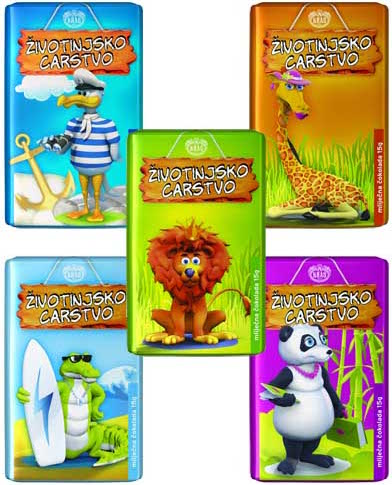
\includegraphics[width=\linewidth]{zivotinjsko-carstvo.jpg}
    \caption{}
\end{marginfigure}

Sličice živali smo že kot otroci lepili v album, nikoli pa nismo zares razumeli, kako so bile karte razporejene po albumu. Kasneje smo se naučili nekaj o taksonomiji, vendar smo inženirji, zato smo jo raje odkrili sami, s podatkovnim rudarjenjem. Taksonomija naj izhaja iz podobnosti (torej merjenja razdalj) med vrstami.

\begin{figure}[h]
    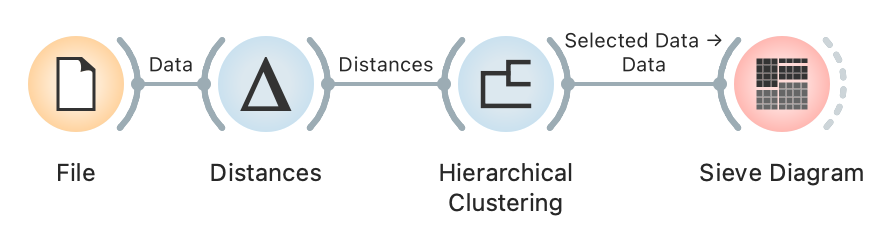
\includegraphics[width=\linewidth]{workflow1.png}%
    \caption{$\;$}
\end{figure}

Uporabili bomo podatke zoo.tab (iz Orangeve dokumentacije). Podatki vsebujejo različne lastnosti živali (ima dlako, ima perje, vali jajca). Izmerimo razdaljo in izračunamo gručenje. Živali v teh podatkih imajo tudi stolpec z razredom, ki mu pripadajo (sesalci, žuželke, ptice, itd.). Ne bi bilo imenitno, če bi gručenje odkrilo te iste razrede? To lahko preizkusimo z gradnikom Hierarchical Clustering, rezultate pa potem opazujemo v Sievovem diagramu.

\begin{figure*}[h]
    \centering
    \newcommand{\clust}{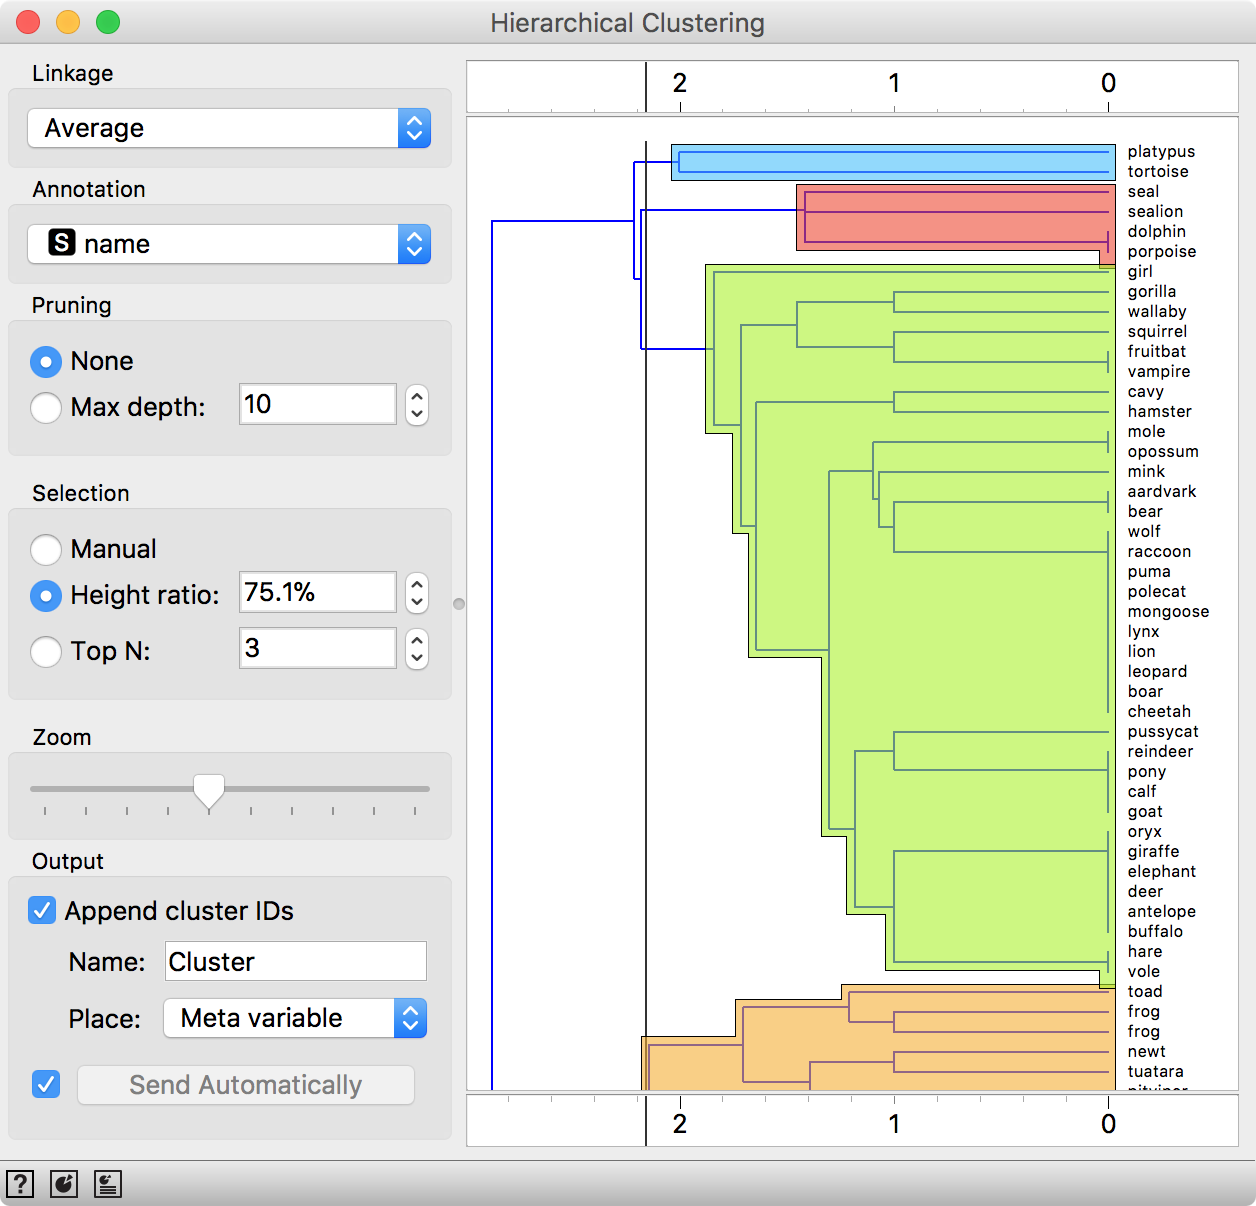
\includegraphics[scale=0.4]{hierarchical-clustering.png}}
    \newcommand{\sieve}{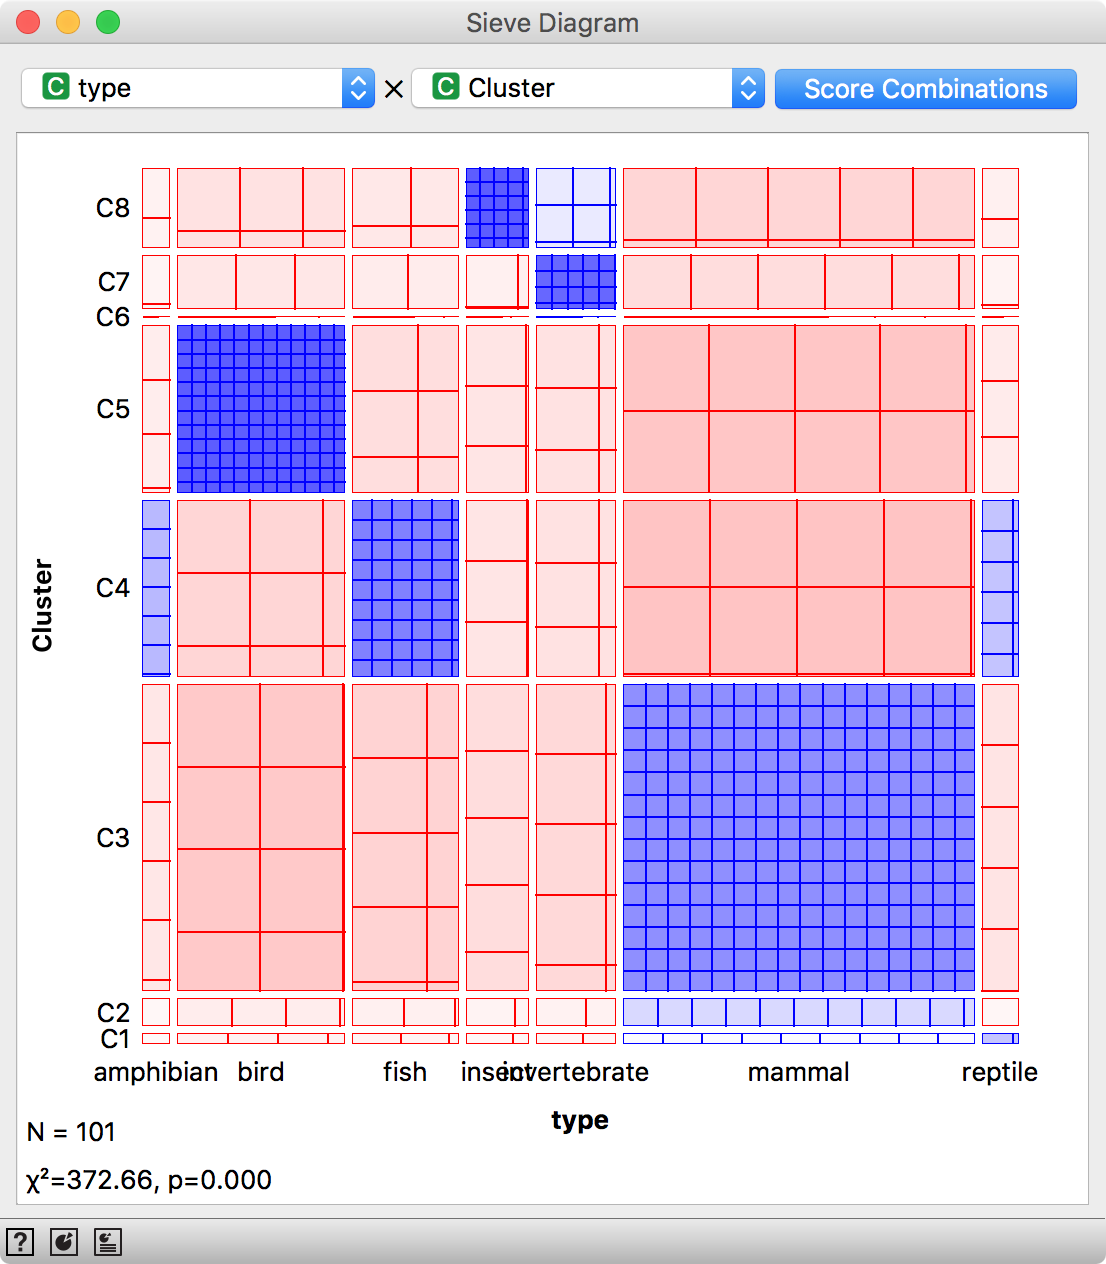
\includegraphics[scale=0.4]{sieve-diagram.png}}
    \infinitewidthbox{
    \stackinset{r}{-0.5\linewidth}{t}{0.0\linewidth}{\sieve}{\clust}\hspace{7cm}
    }
\end{figure*}

\newpage

Rezultati so zanimivi. Vse ptice, na primer, je gručenje prepoznalo kot eno skupino (označilo jo je s C6). Skupina C4 pa je mešana in vsebuje dvoživke, ribe in plazilce.

\begin{figure}[h]
    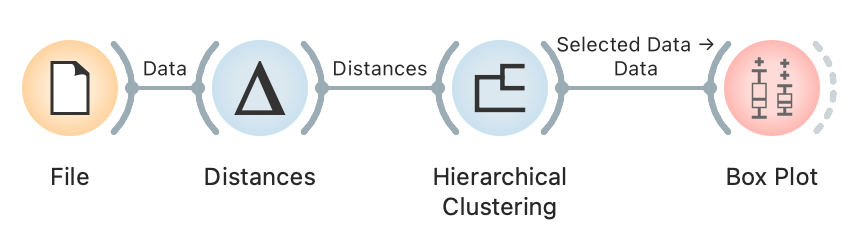
\includegraphics[width=\linewidth]{workflow2.png}%
    \caption{$\;$}
\end{figure}

Še lepše je, če to pogledamo v gradniku \widget{Box Plot}. Vidimo lahko porazdelitev razredov živali po izbranih gručah. Ali pa vizualizacijo obrnemo in pogledamo, v katerih gručah so kateri razredi.

\begin{figure}[h]
    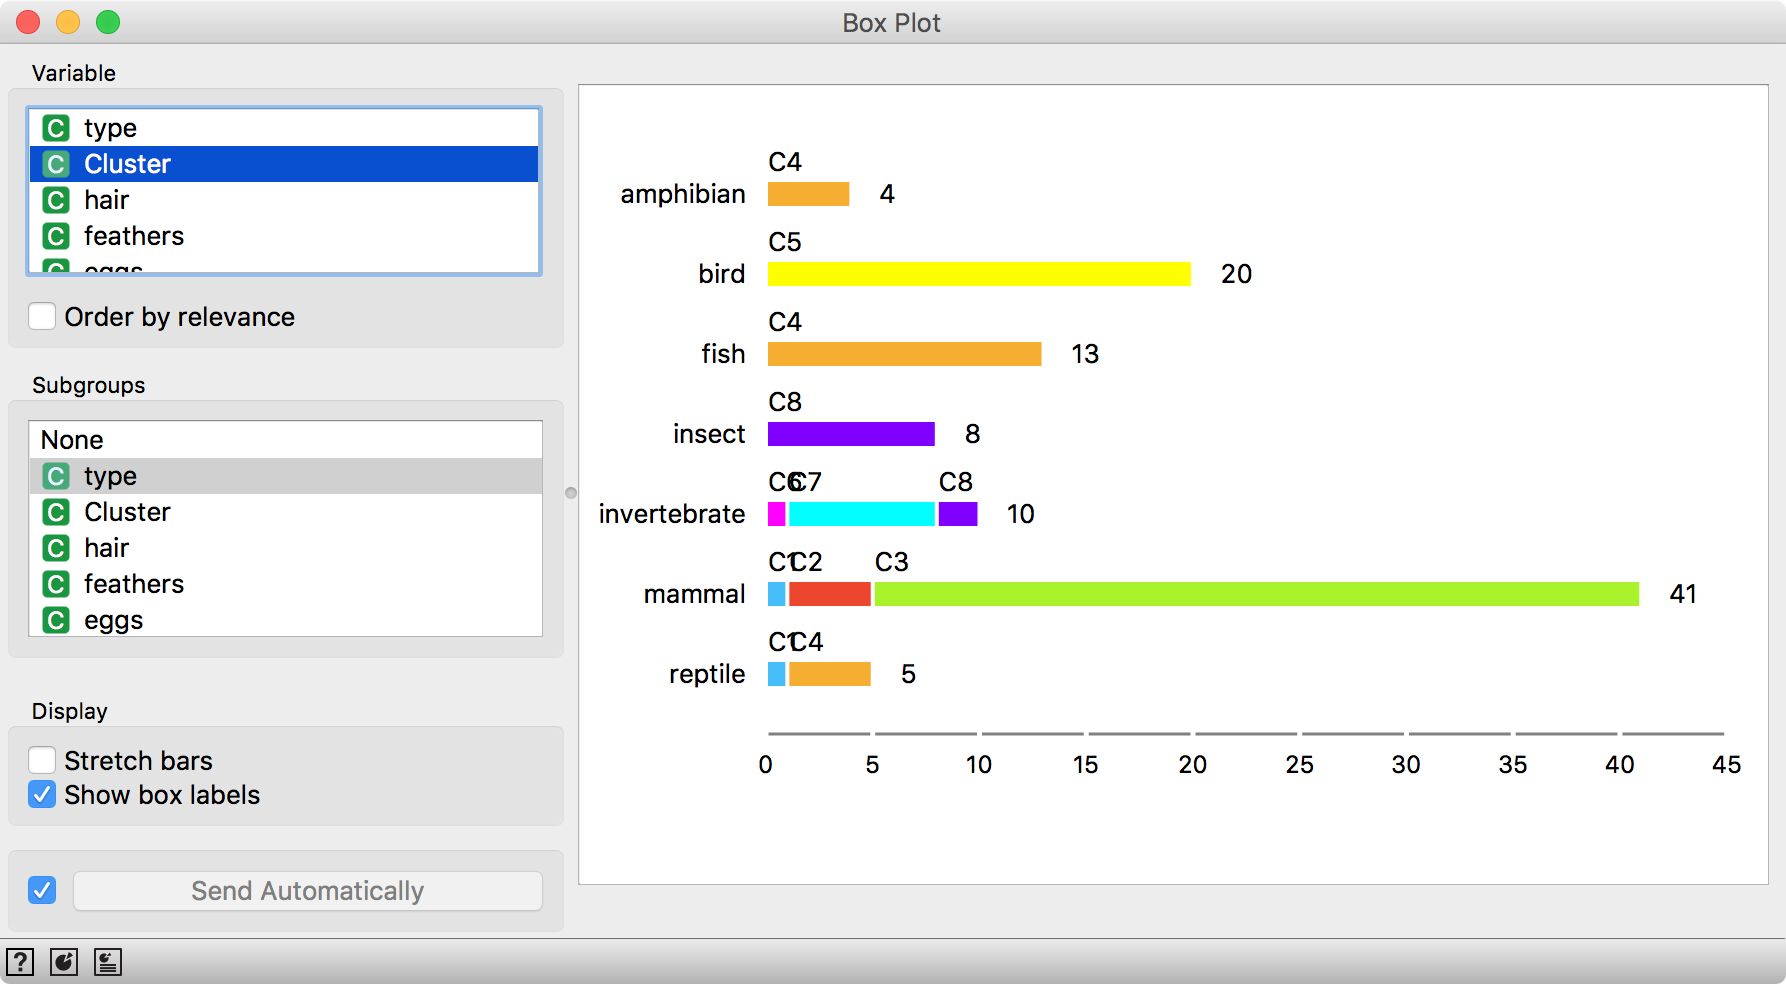
\includegraphics[width=\linewidth]{box-plot.png}%
    \caption{$\;$}
\end{figure}

Kaj pa je narobe s sesalci? Zakaj niso v eni sami skupini? Za to sta dva razloga. Prvi je, da predstavljajo kar 40\% primerov. Drugi pa, da vsebujejo nekaj čudakov. Izberite skupino v škatli z brki in preverite, katere živali so to.

Posebnosti izbranih skupin lahko preverimo tako, da gradniku Box Plot odkljukamo opcijo ‘Order by relevance’, v Subgroups razdelku pa izberemo zopet spremenljivko Cluster. Očitno se skupine zares najlepše ločijo po razredih živali. Kako zanimivo!

\newpage

\begin{figure}[h]
    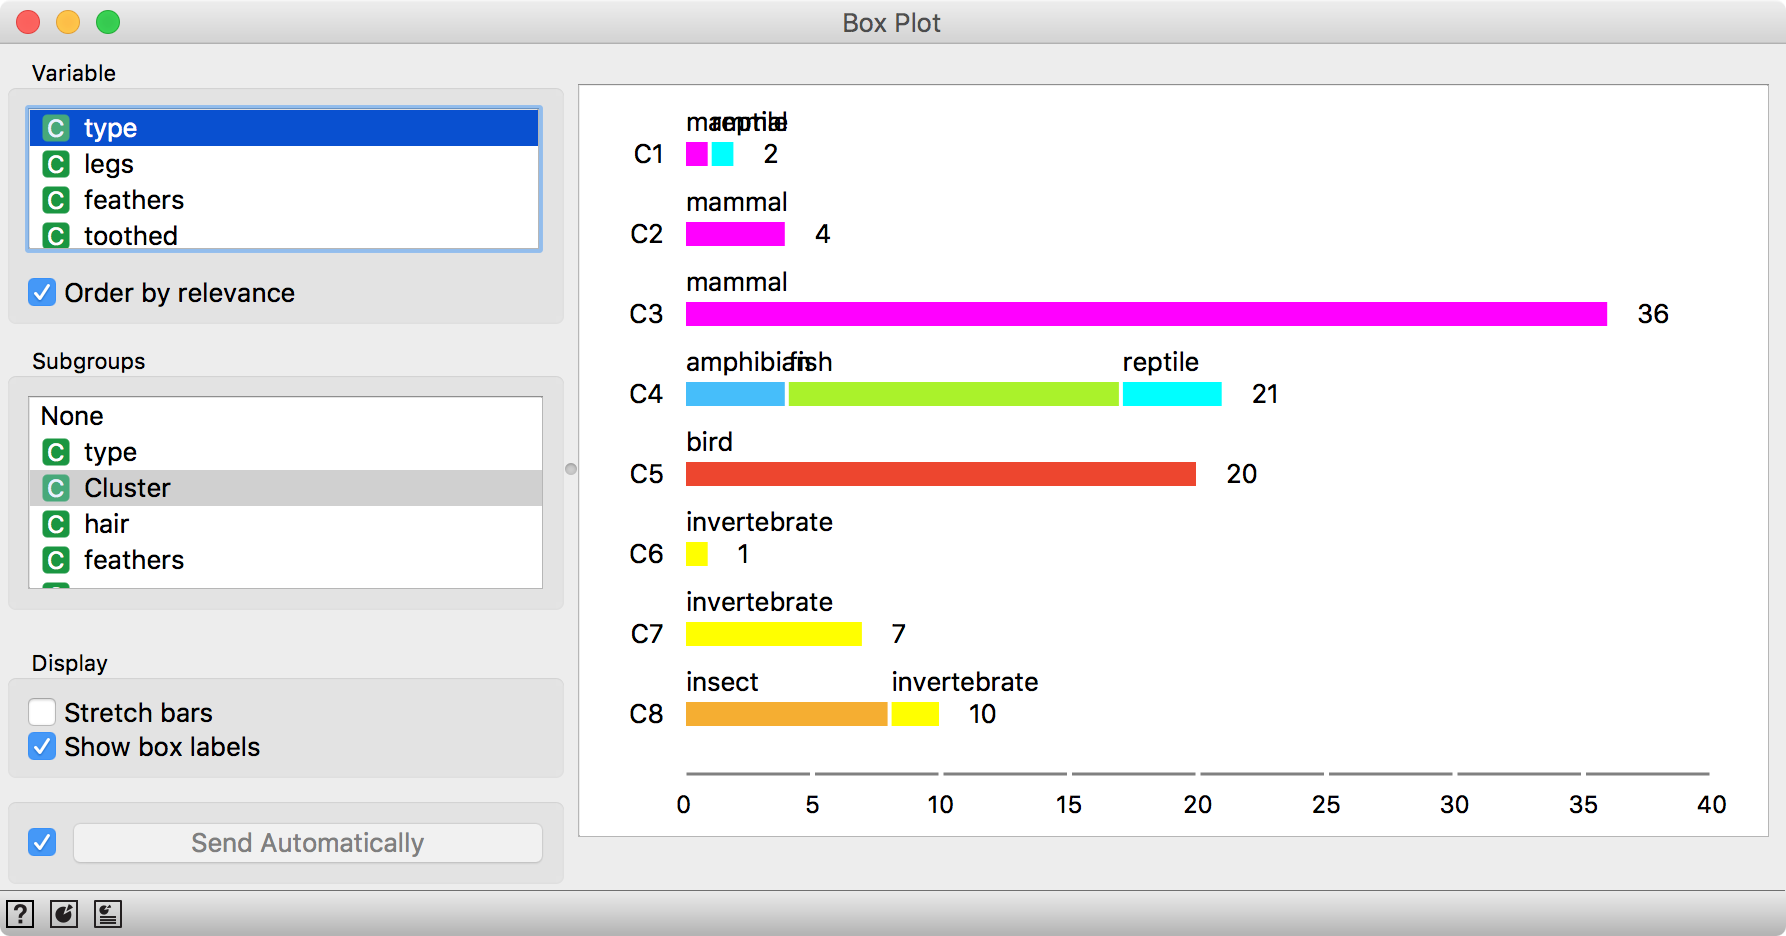
\includegraphics[width=\linewidth]{box-plot2.png}%
    \caption{$\;$}
\end{figure}

\begin{marginfigure}[1.5cm]
    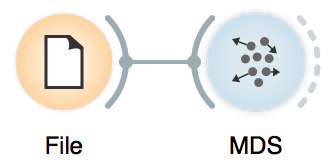
\includegraphics[width=\linewidth]{workflow3.png}
    \caption{}
\end{marginfigure}

S pomočjo hierarhičnega razvrščanja težko vidimo, kako podobna sta si, npr. želva in pingvin. Za to obstaja vizualizacija, ki primeri, ki so si med seboj podobni, nariše blizu skupaj, različne pa daleč. Tako vizualizacijo imenujemo večrazsežnostno lestvičenje (multidimensional scaling, MDS).

\begin{figure*}[h]
    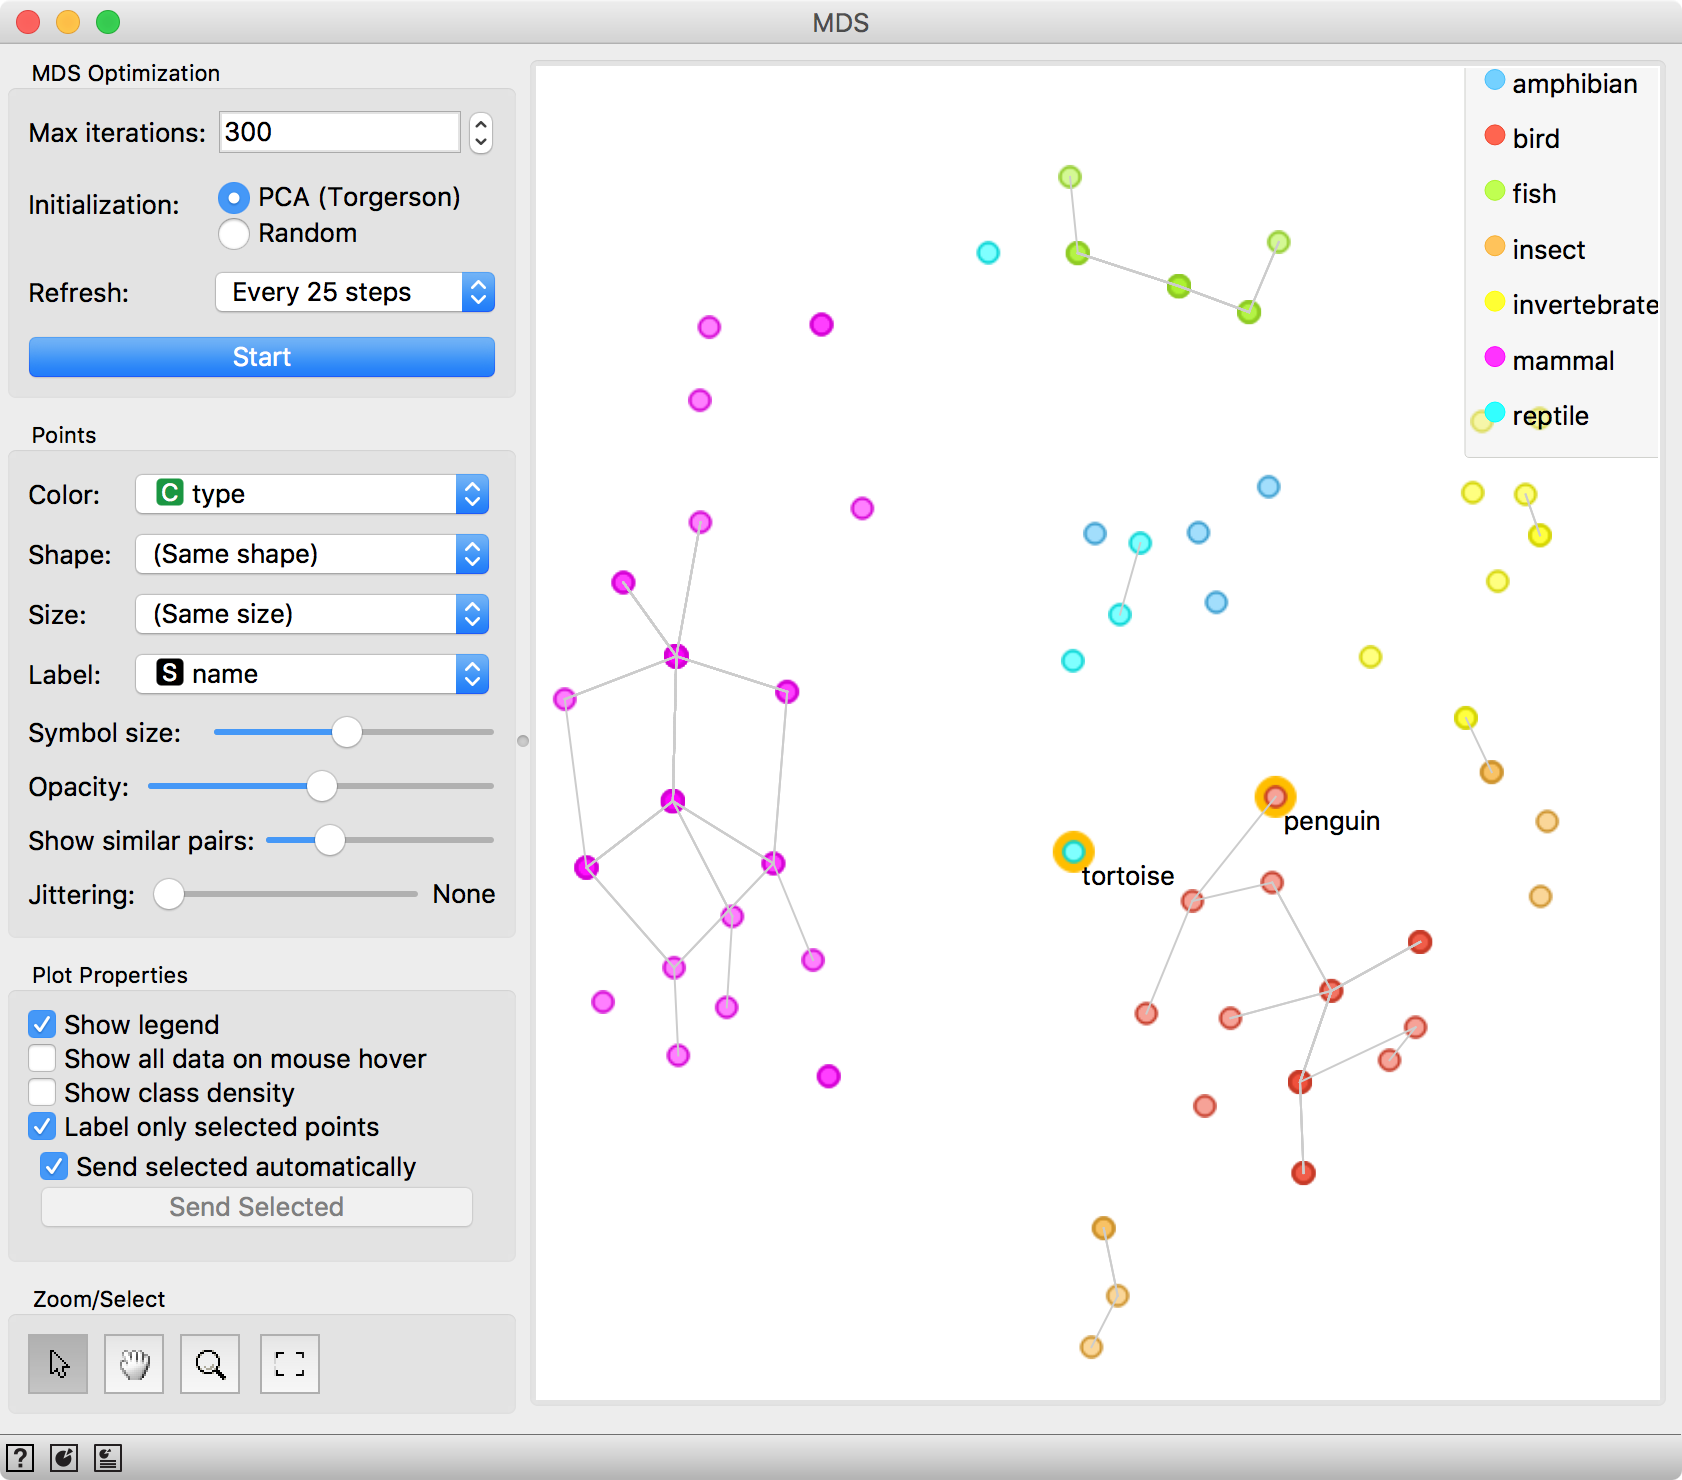
\includegraphics[width=0.7\linewidth]{mds.png}%
    \caption{$\;$}
\end{figure*}